
\section{Theorie}
\label{sec:Theorie}
Wenn Gamma-Strahlung Materie durchdringt wird ein Teil der Strahlung materialabhängig absorbiert und die abgeschwächte Intensität kann gemessen werden. Aus verschiedenen Messungen einer Schicht, die aus unterschiedlichen Richtungen erfolgen, entstehen bei einer Tomographie Projektionen, die schlussendlich zu einem 2D-Bild zusammen gesetzt werden können. Unter einer Projektion versteht man die Durchstrahlung eines Körpers mit einer bestimmten Ausrichtung. \\
\subsection{Wechselwirkung von Strahlung mit Materie}
In diesem Versuch wird ${}^{137}\mathrm{Cs}$ als Strahlungsquelle verwendet. Dies zerfällt zu 94,6\% in ${}^{137}\mathrm{Ba}$. Dies ist danach im angeregten Zustand. Um in den Grundzustand zu gelangen, entsendet es ein Photon mit der Energie von $\SI{661,6}{\kilo\electronvolt}$ \cite{Anleitung5}. In Abbildung (\ref{fig:caes}) ist dies dargestellt.
\begin{figure}
	\centering
	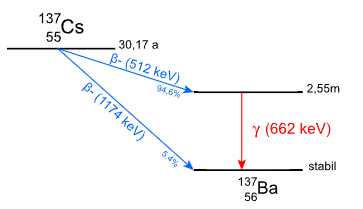
\includegraphics[scale=0.7]{fig/caes.png}
	\caption{Zerfall von ${}^{137}\mathrm{Cs}$ \cite{leifi}.}
	\label{fig:caes}
\end{figure}
\FloatBarrier
\noindent Die Absorption der Photonen erfolgt durch drei unterschiedlichen Effekte. Diese sind der Photo-Effekt, der Compton-Effekt und die Paarbildung.
\begin{itemize}
	\item Beim Photoeffekt trifft ein Photon auf ein Hüllenelektron und gibt dabei seine Energie $E_\mathrm{\gamma}$ vollständig an das Elektron ab. Dieses wird daraufhin
	aus der Hülle gelöst. Die Bedingung für den Effekt ist, dass die Energie des Photons größer ist als die Bindungsenergie des Elektron, also $E_\gamma>E_\mathrm{Bindung}$.
	\item Beim Compton-Effekt werden die einfallenden Photonen inelastisch an Elektronen gestreut. Im Gegensatz zum Photoeffekt wird dabei wird nur ein Teil der Energie abgegeben.
 	\item Bei der Paarbildung zerfällt das Photon unter Einfluss des Coulomb-Feldes des Atomkerns in ein Elektron und ein Positron. Dabei muss die Energie des Photons aufgrund der Energieerhaltung mindestens $E=\SI{1,02}{\mega\electronvolt}$ betragen, dies entspricht der Ruhemasse von zwei Elektronen.
\end{itemize}
\FloatBarrier
\noindent Die drei Fälle unterscheiden sich in ihrer Häufigkeit im Verhältnis zur Energie.
Während der Photo-Effekt bei Energien bis $\SI{100}{\kilo\electronvolt}$ dominiert, tritt der Compton-Effekt von $\SI{100}{\kilo\electronvolt}$ bis $\SI{1}{\mega\electronvolt}$ auf. Die Paarbildung ist der stärkste Effekt ab einer Energie $E=\SI{1}{\mega\electronvolt}$.
Die Intensität nach dem Durchqueren des Materials kann über das Absorptionsgesetz beschrieben werden, als:
\begin{align}
  \label{eqn:Ab}
  I=I_\mathrm{0} \exp\left(\sum_i \mu_\mathrm{i} d_\mathrm{i}\right)
\end{align}
Dabei ist $I$ die gemessene Intensität nach Durchquerung von Materie, $I_\mathrm{0}$ die Anfangsintensität, $\mu_\mathrm{i}$ der Absorptionskoeffizient, sowie $d_\mathrm{i}$ die Dicke des i-ten Materials.
Ein Spektrum der ${}^{137}\mathrm{Cs}$ Strahlung besteht im niedrigen Energiebereich aus Rückstreuung, das nachfolgende Minimum ist die sogenannte Compton-Kante. Der darauffolgende Peak ist der Photo-Peak. In Abbildung (\ref{fig:spekt}) ist das Gammaspektrum von ${}^{137}\mathrm{Cs}$ dargestellt.
\begin{figure}
	\centering
	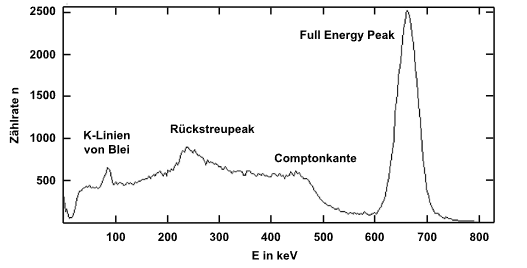
\includegraphics[scale=0.7]{fig/spek_cs.png}
	\caption{Gammaspektrum von ${}^{137}\mathrm{Cs}$ \cite{leifi}.}
	\label{fig:spekt}
\end{figure}
\FloatBarrier
\subsection{Bestimmung der Absorptionskoefizienten}
\noindent Durch Umstellung der Gleichung (\ref{eqn:Ab}) folgt:
\begin{align}
  \label{eqn:umab}
  \sum\limits_{i}^{}\mu_\mathrm{i} d_\mathrm{i} = \ln\left(\dfrac{I_\mathrm{0}}{I}\right)
\end{align}
Durch Zusammenfassen aller Dicken $d_\mathrm{i}$ in eine Geometriematrix $A$, aller Absorptionskoeffizienten $\mu$ in einen Vektor $\vec{\mu}$ und dem Vektor $\vec{I}$, der alle Verhältnisse zwischen $I$ und $I_\mathrm{0}$ enthält, ergibt sich:
\begin{align}
  \label{egn:Matrixschreibweise}
  A \vec{\mu} = \vec{I}
\end{align}
Um das Gleichungssystem zu lösen und den Fehler so klein wie möglich zu halten, muss das Gleichungssystem überbestimmt sein, weiter wird die Methode der kleinsten Quadrate genutzt. Daraus folgt:
\begin{align}
  \label{eqn:Quadrate}
  W A \vec{\mu} = W \vec{I}
\end{align}
Mit der Gewichtungsmatrix $W=V[\vec{I}]^{-1}$, wobei $V$ die Unsicherheit angibt, ergibt sich:
\begin{align}
  \label{eqn:letzte Gleichung}
  \vec{\mu}=\left(A^TWA\right)^{-1}\left(A^TW\vec{I}\right)
\end{align}
Die Unsicherheiten sind gegeben durch:
\begin{equation}
  V[\vec{\mu}]=\left(A^TWA\right)^{-1}
  \label{eqn:mu}
\end{equation}
